
\begin{enumerate}
    \item Two loudspeakers \(M\) and \(N\) are located 20 m apart and emit sound at frequencies 118 Hz and 121 Hz, respectively. A car is initially at a point \(P\), 1800 m away from the midpoint \(Q\) of the line \(MN\) and moves towards \(Q\) constantly at 60 km/hr along the perpendicular bisector of \(MN\). It crosses \(Q\) and eventually reaches a point \(R\), 1800 m away from \(Q\). Let \(v_P\), \(v_Q\) and \(v_R\) be the beat frequencies measured by a person sitting in the car at time \(t\). Let \(v(t)\) represent the beat frequency measured by a person sitting in the car at time \(t\). The speed of sound in air is 330 m s\(^{-1}\). Which of the following statement(s) is(are) true regarding the sound heard by the person?
        \begin{tasks}(1)
            \task \(v_P + v_R = 2 v_Q\)
            \task The rate of change in beat frequency is maximum when the car passes through \(Q\)
            \task The plot below represents schematically the variation of beat frequency with time (with a labeled diagram indicating points \(P\), \(Q\), and \(R\).)
            \task The plot below represents schematically the variation of beat frequency with time (with a labeled diagram indicating points \(P\), \(Q\), and \(R\).)
        \end{tasks}
\end{enumerate}
\begin{center}
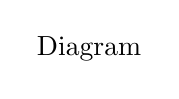
\begin{tikzpicture}
\node {Diagram};
\end{tikzpicture}
\end{center}
